\section{User Manual}
\label{usermanual}

\subsection{How to Install the game}
The game can be run on either an Android device, smart phone or tablet, or
the Android emulator on a laptop.

Note that all screenshots are not of actual size.

In order to install the game on an Android device, follow these instructions
\begin{enumerate}
\item Copy the apk file to your Android's memory card and insert the card to
your device
\item Download and install the apk Installer from Google Play\cite{website:apk}
\item Once installed, the apk Installer will display the apk files on the
memory card
\item Click and install the bepresbingo.apk file
\item Wait for installation 
\item Launch `Bedpres Bingo' by pressing the icon in the menu
\end{enumerate}

\subsection{How to play Bedpres-Bingo}

\subsubsection{Start new game}
In order to initiate a new game, the player will press the New Game-button.
\begin{center}
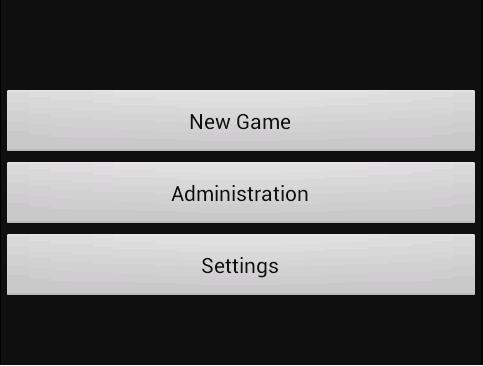
\includegraphics{Pikks/mainmenu}
\captionof{figure}{Main menu}
\end{center}

\subsubsection{Playing Bedres-bingo}
The main gameplay will be played on the Bingo Board shown below. The game
should be played in context of a `Bedpres' in order to be played properly.
The speaker will be the one presenting words. When a player hears a specific
word, the player presses the corresponding word on his/her device.

When a word is pressed, the cell with the word will turn green. The goal is to
cross off all the words in a row or column. The game is ultimately won by
crossing off all the words on the board.

In ``Bedpres-Bingo'', there are several goals. The name of the person
getting to each of the goals will be announced.
The goals are ranged as following:
\begin{enumerate}
	\item{Golden MegaBingo}
	\item{MegaBingo}
	\item{Golden TripleBingo}
	\item{Triplebingo}
	\item{Golden DoubleBingo}
	\item{DoubleBingo}
	\item{Golden SingleBingo}
	\item{SingleBingo}
\end{enumerate}


\begin{center}
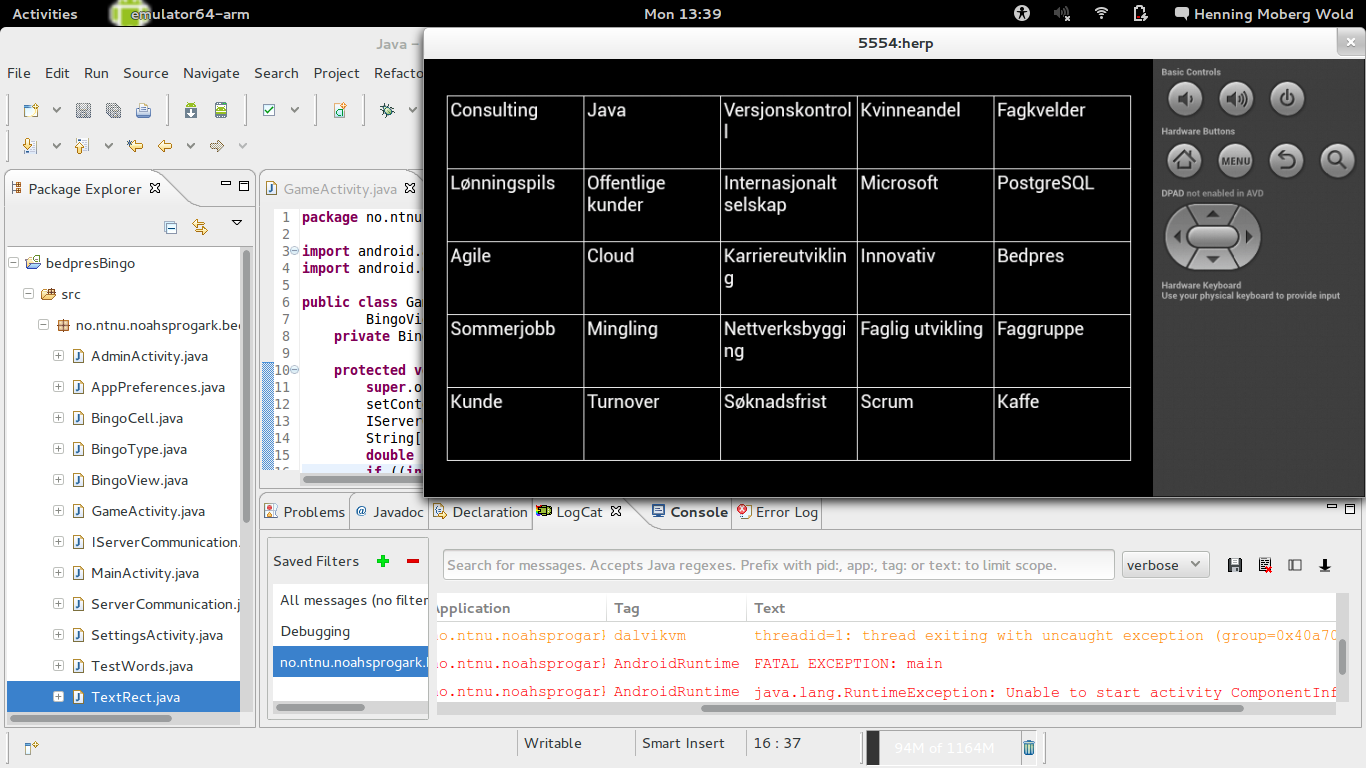
\includegraphics[scale=0.6]{Pikks/maingame}
\captionof{figure}{Main game board}
\end{center}

\subsubsection{Change your name}
In accordance with FR2: ``Set player names'', the players should be able to
change their name. This is done via the settings menu. The player may enter a
name, and press the OK-button in order to change the name that will be used
in-game.

\begin{center}
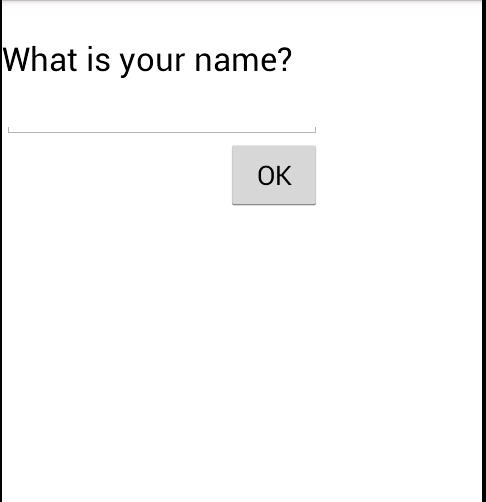
\includegraphics{Pikks/settings}
\captionof{figure}{Settings screen}
\end{center}
